\chapter{Aporte de Franshesco: refactorización del backend y avisos internos}
\label{cap:franshesco}

\section{Objetivo, responsabilidad y referencia inicial}
El aporte de Franshesco, Scrum Master y desarrollador backend, consiste en mejorar
la organización de usuarios, autenticación y permisos, e implementar avisos internos
desacoplados de las capacitaciones. El trabajo se realiza sobre la aplicación
funcional existente, conservando las contribuciones del equipo. La implementación,
las pruebas y esta documentación se desarrollaron con asistencia de Codex; la
revisión humana y la validación de las reglas con Paz Sur son actividades distintas.

La referencia \textbf{Punto Inicio Fran} es la etiqueta anotada
\texttt{punto-inicio-fran}, sobre el commit \texttt{98f8d5a}. Esta base ya incorpora
el frontend de usuarios y roles de Brenda y la separación del backend de
capacitaciones de Adel. No se atribuyen esos cambios a Franshesco ni se integra
automáticamente la rama pendiente de Daniela. El punto final se identifica por
el mensaje de commit \textbf{Punto final fran 1}, en \path{dev/franshesco}.

El alcance se relaciona con HU-01 (usuarios), HU-02 (permisos y roles), HU-16
(autenticación) y una ampliación parcial de HU-26 (avisos), conectada con HU-03/04.
Se distinguen dos tipos de trabajo: \textbf{refactorización}, que conserva los
contratos existentes al separar responsabilidades, y \textbf{ampliación funcional},
que añade eventos, persistencia y bandeja de avisos. No se implementan autorregistro,
login por nombre de usuario, envío de credenciales ni mensajería por WhatsApp.

\section{Diagnóstico del código anterior}
La base ya contaba con validación Zod, SQL parametrizado, hashes scrypt, sesiones
opacas en cookie HttpOnly, protección CSRF, auditoría y reglas administrativas.
La mejora no consiste en presentar esos mecanismos como nuevos, sino en organizar
sus responsabilidades y corregir puntos concretos de autorización y mantenimiento.

\begin{table}[htbp]
\centering\small
\begin{tabular}{P{0.44\textwidth}P{0.48\textwidth}}
\toprule Problema observado & Cambio realizado \\ \midrule
El servicio de usuarios reúne esquemas, reglas, hashing y SQL. & Extraer validación, políticas, servicios y repositorios específicos. \\
La ruta de login coordina credenciales, límite de intentos y sesiones. & Delegar el caso de uso a un servicio; mantener HTTP y cookies en la ruta. \\
La autorización de usuarios se consulta antes de esperar el hash. & Revalidar actor y objetivo dentro de la transacción posterior a la espera. \\
La modificación de roles confía en la autorización de la ruta. & Exigir el permiso también dentro del servicio. \\
El listado hidrata cada persona mediante consultas adicionales. & Recuperar perfiles, roles y permisos por lote. \\
El manejador identifica duplicados buscando texto en errores. & Traducir códigos SQLite y proteger los detalles de errores inesperados. \\
No existe un consumidor de eventos de capacitaciones. & Añadir Observer y una bandeja interna con recuperación de pendientes. \\
\bottomrule
\end{tabular}
\caption{Diagnóstico y solución sobre Punto Inicio Fran.}
\end{table}

Antes de cambiar el código, la referencia aprobó 75 pruebas de backend y cuatro
escenarios de navegador. Esta comprobación sirve de base de regresión; no demuestra
que las funcionalidades nuevas ya existieran.

\section{Arquitectura y aplicación de SOLID}
Se conserva un \textbf{monolito modular por capas}: React presenta la interfaz;
las rutas Express reciben solicitudes y autorizan; los servicios coordinan casos
de uso; los repositorios contienen SQL; SQLite conserva los datos y restricciones.
La aplicación continúa usando una API de misma procedencia, sin microservicios ni
dependencias nuevas.

\begingroup\setlength{\parskip}{0pt}
\begin{longtable}{P{0.27\textwidth}P{0.65\textwidth}}
\toprule Responsabilidad & Archivos representativos \\ \midrule\endhead
Entradas y filtros & \path{server/validation/user-validation.js}, validadores de autenticación y notificaciones. \\
Reglas de acceso & \path{server/authorization/user-policy.js}. \\
Casos de uso & \path{server/services/user-management.js}, \path{role-service.js}, \path{auth-service.js}. \\
Persistencia & Repositorios de usuarios, roles, sesiones, auditoría, eventos y notificaciones en \path{server/repositories/}. \\
Seguridad técnica & Credenciales, restauración de sesión y límite de intentos en \path{server/auth/}. \\
Conexión de módulos & \path{server/composition.js} y composición del módulo de notificaciones. \\
Compatibilidad & \path{server/services/user-service.js} y \path{server/security.js} conservan fachadas para consumidores previos. \\
\bottomrule
\end{longtable}\endgroup

\textbf{SRP, responsabilidad única.} La validación describe entradas admisibles;
la política determina autorización; el servicio coordina reglas y transacciones;
el repositorio ejecuta consultas. Esto aumenta la cohesión: cada módulo agrupa
operaciones relacionadas con una responsabilidad concreta.

\textbf{DIP, inversión de dependencias.} Los casos de uso reciben objetos con las
operaciones necesarias: repositorios, hashing, reloj, auditoría y transacción.
No importan Express ni SQLite. El punto de composición conecta esas operaciones
con implementaciones concretas. Se reduce así el acoplamiento entre negocio y
tecnología, y las pruebas pueden sustituir colaboradores con objetos en memoria.
La inyección de dependencias es la técnica utilizada para materializar esa separación.

No se afirma que cambiar de motor sea automático: el SQL y las transacciones
seguirían necesitando adaptación. Tampoco se declara la aplicación de todos los
principios SOLID por el simple hecho de dividir archivos.

\section{Registro y edición de usuarios: antes y después}
La función anterior mezcla validación, autorización, hashing y escritura SQL. El
fragmento se obtuvo mediante \texttt{git show} sobre la referencia inicial, sin
reconstrucción manual.

\lstinputlisting[language=JavaScript,firstline=53,lastline=69,basicstyle=\ttfamily\scriptsize,caption={Antes: varias responsabilidades dentro de createUser.}]{codigo/franshesco/antes/user-service.js}

En la versión refactorizada, el servicio conserva la coordinación del caso de uso,
pero delega cada responsabilidad. La segunda autorización se realiza después del
\texttt{await}, dentro de la transacción, para impedir una escritura si el permiso
fue revocado durante el cálculo del hash.

\lstinputlisting[language=JavaScript,firstline=26,lastline=40,basicstyle=\ttfamily\scriptsize,caption={Después: coordinación mediante colaboradores inyectados.}]{codigo/server/services/user-management.js}

Perfil, roles y auditoría siguen formando una operación atómica. Se conservan
correo y documento únicos, normalización del correo, reglas de contraseña y
revocación de sesiones al cambiar la contraseña o desactivar una cuenta.
El valor de actor nulo sólo se usa desde la semilla local; ninguna ruta pública
permite omitir al actor para administrar usuarios.

La comparación de código 01 muestra esta extracción y la 05 muestra cómo
\path{composition.js} entrega las implementaciones. La comparación visual 04
confirma que se conserva el formulario de Brenda; la 05 muestra el rechazo real
de correo duplicado con respuesta 409, comportamiento que ya existía.

\begin{figure}[htbp]\centering
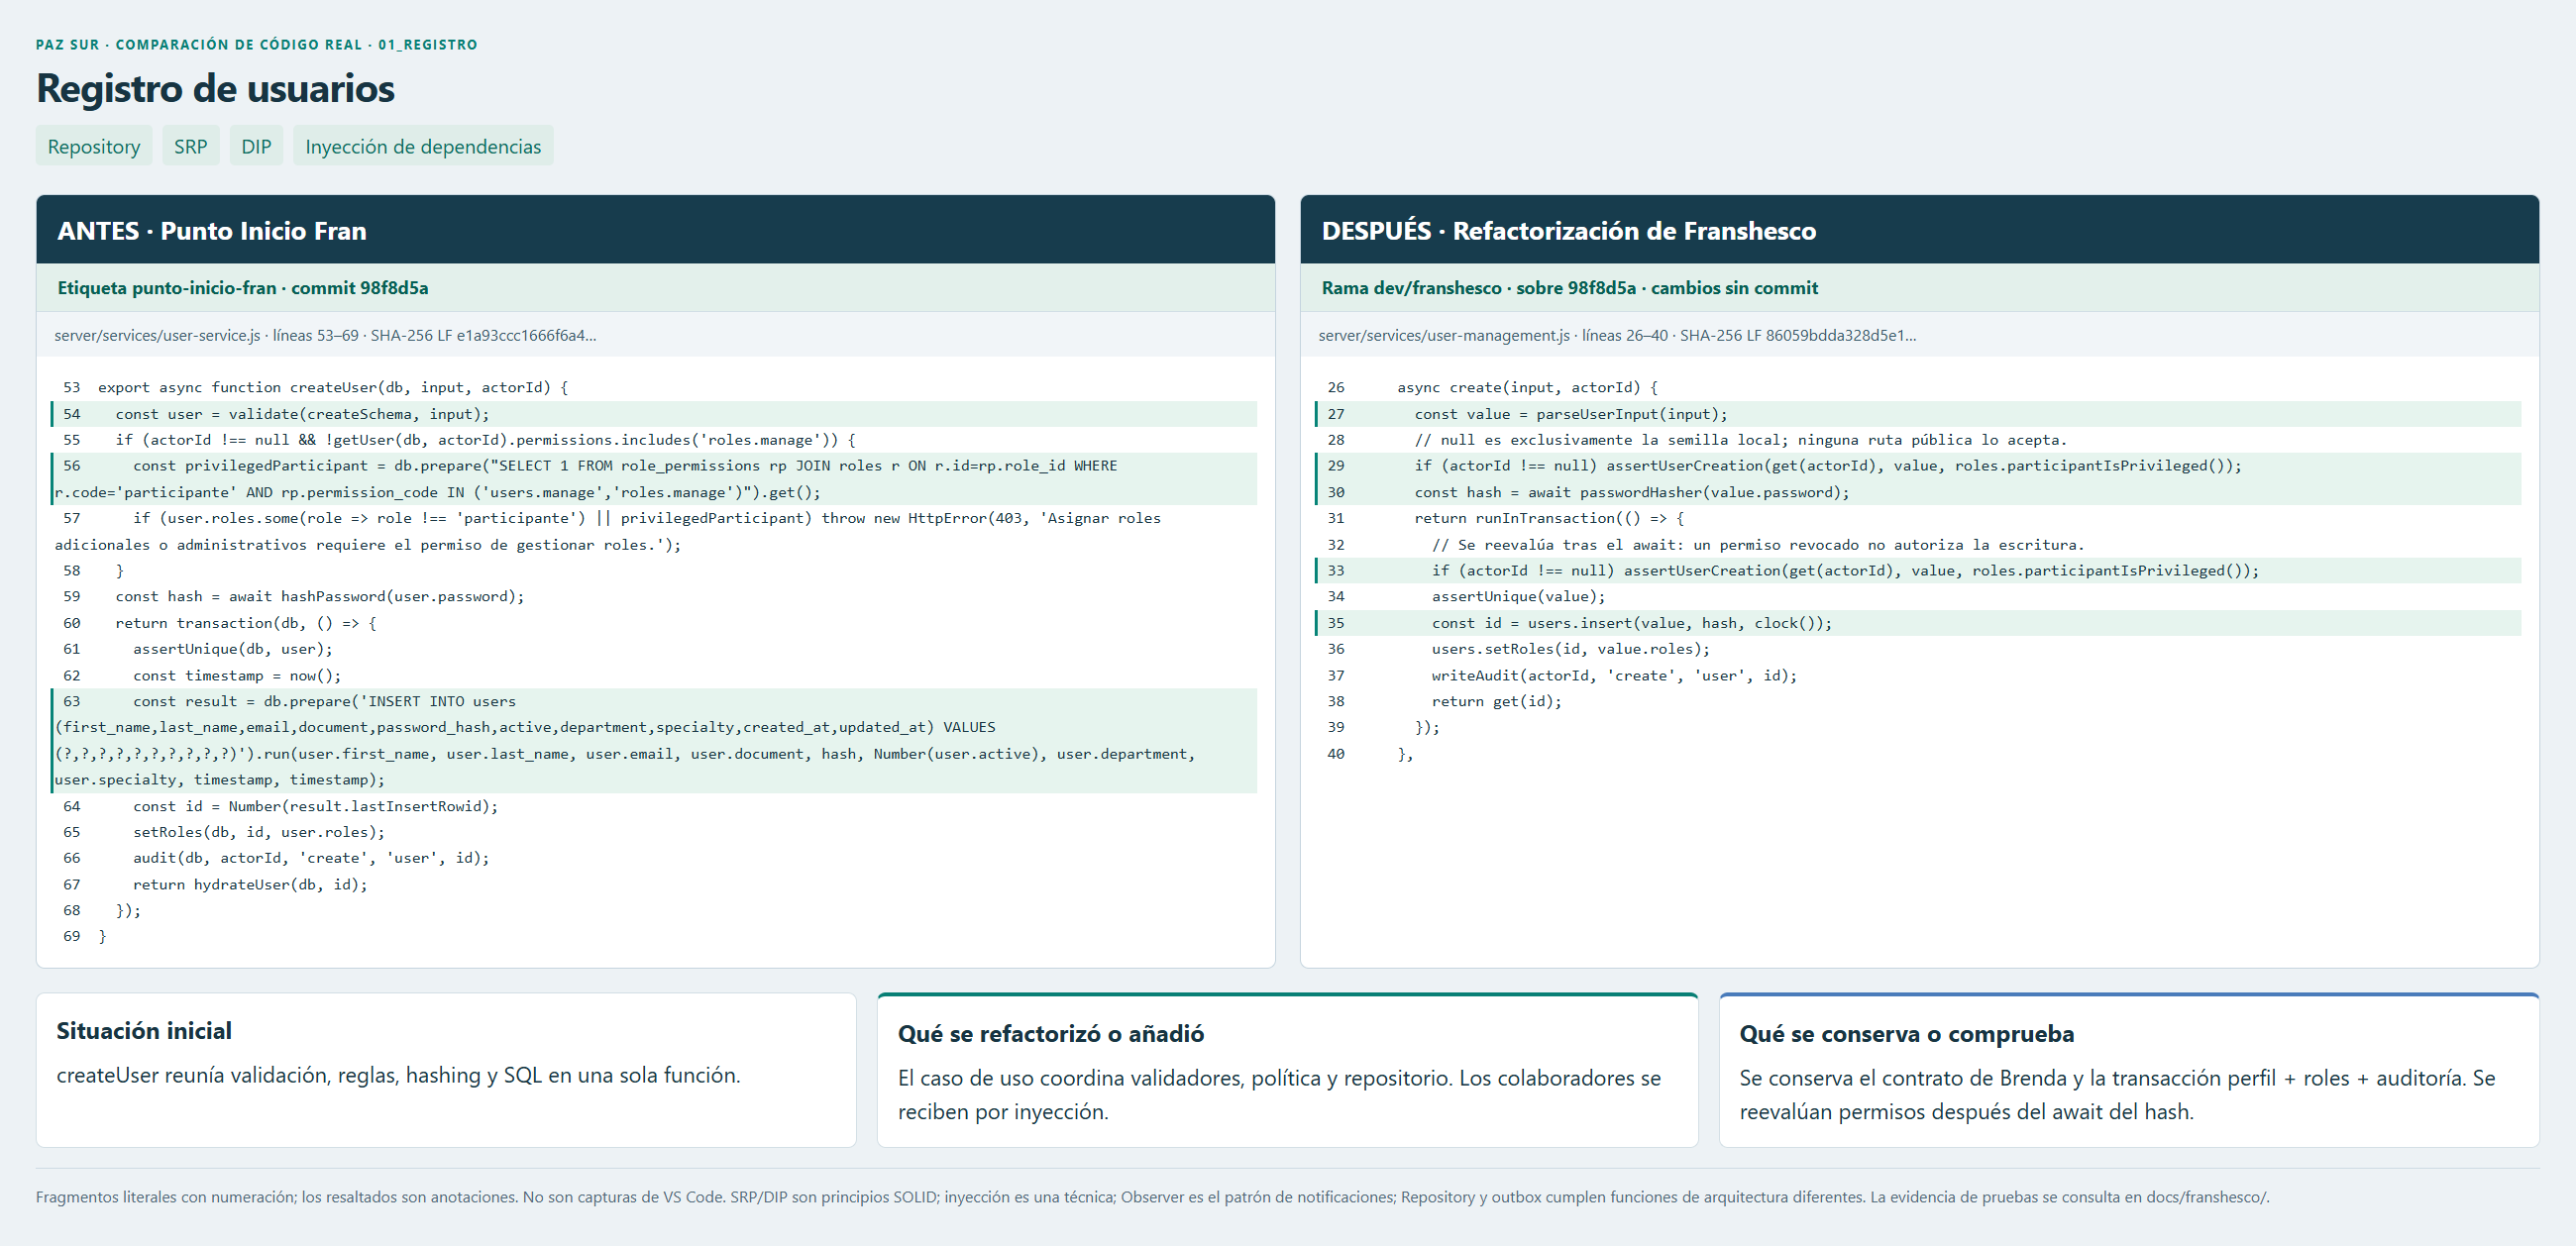
\includegraphics[width=\linewidth,height=0.82\textheight,keepaspectratio]{imagenes/franshesco/comparacion_codigo_01_registro.png}
\caption{Registro: código real anterior y refactorizado, con archivos, líneas, versiones y explicación de diseño. Las láminas originales permiten ampliar los detalles.}
\end{figure}

\section{Autenticación, permisos y tratamiento de errores}
\subsection{Autenticación}
El login continúa recibiendo correo y contraseña. El servicio valida la entrada,
aplica el límite de intentos, consulta credenciales y verifica scrypt. Después de
esa espera comprueba nuevamente que la cuenta siga activa y conserve el mismo
hash; sólo entonces crea la sesión y su auditoría. La ruta devuelve la cookie y
la respuesta HTTP, sin ejecutar SQL.

Se conservan la cookie HttpOnly, SameSite, vencimiento, token opaco almacenado como
hash y CSRF para mutaciones autenticadas. Los permisos se recuperan de la base en
cada solicitud, evitando guardar privilegios desactualizados en la cookie. El
límite de intentos sigue siendo local al proceso; no se presenta como protección
distribuida. Las comparaciones de código 02 y visual 01 muestran que cambia la
estructura interna mientras se mantiene la experiencia de ingreso.

\subsection{Autorización}
Las comprobaciones de las rutas se conservan y las operaciones sensibles refuerzan
sus reglas dentro del servicio. Ocultar un botón no constituye autorización.

\begin{table}[htbp]\centering\small
\begin{tabular}{P{0.32\textwidth}P{0.60\textwidth}}
\toprule Permiso o regla & Comportamiento comprobado \\ \midrule
\texttt{users.manage} & Permite gestionar perfiles; por sí solo no concede gestión de roles ni edición de cuentas administrativas. \\
\texttt{roles.manage} & Autoriza asignaciones de roles y modificación de permisos; el servicio lo exige incluso en llamadas directas. \\
Administrador protegido & No se retira el último administrador activo ni se modifica la configuración del rol administrador. \\
Permisos actuales & Una revocación afecta solicitudes posteriores y se revalida antes de escribir después del hashing. \\
Propiedad de avisos & Cada persona consulta y marca sólo sus avisos cuyo alcance de capacitación siga vigente. \\
\bottomrule
\end{tabular}
\caption{Reglas de autorización conservadas y reforzadas.}
\end{table}

La delegación de usuarios sin gestión de roles sólo admite altas con rol
participante sin privilegios administrativos indirectos. Varios argumentos de
\texttt{requirePermission} significan cualquiera de ellos (OR), conservando el
contrato anterior. Las comparaciones de código 03 y visuales 06--08 se relacionan
con estas reglas; la autorización efectiva se comprueba mediante pruebas de API
y servicios, no por la apariencia de los formularios.

\subsection{Errores}
Se mantiene el contrato \texttt{\{error:\{message,fields?\}\}}. Los códigos distinguen
sesión ausente (401), autorización o CSRF (403), registro no disponible (404),
conflicto (409), validación (422), límite de intentos (429) y fallo inesperado (500).
El manejador separado traduce códigos SQLite de unicidad, relaciones, restricciones
y bloqueo; este último se comunica como 503. Los detalles de campos sólo se
devuelven en errores controlados, y los fallos inesperados mantienen un mensaje
genérico. La comparación de código 09 muestra el cambio; no requiere añadir
artificialmente otro patrón de diseño.

\section{Repository y mejora del listado}
Los repositorios separan SQL de los casos de uso. Además de facilitar el
mantenimiento, el repositorio de usuarios elimina consultas repetidas por persona.
Antes se consultaban IDs y se hidrataba cada perfil mediante tres SELECT; después
se recuperan conteo, perfiles, roles y permisos por lote, preservando paginación,
orden y ausencia de hashes en las respuestas.

\begin{center}\begin{tabular}{lrr}
\toprule Medición del listado & Antes & Después \\ \midrule
Cuentas ficticias en la base & 404 & 404 \\
Personas por página & 100 & 100 \\
SELECT, excluyendo autenticación & 302 & 4 \\
\bottomrule
\end{tabular}\end{center}

La medición se obtuvo en ambas versiones con cuatro cuentas de semilla y 400
adicionales. Una página vacía sólo requiere dos consultas. La comparación de
código 04 y los manifiestos registran esta mejora estructural; no se atribuye
una reducción de tiempo no medida ni capacidad para 400 conexiones simultáneas.

\section{Observer: avisos sin acoplar capacitaciones a notificaciones}
\subsection{Problema y participantes del patrón}
La versión inicial guardaba capacitaciones sin generar avisos. Añadir una llamada
directa a un canal desde el servicio mezclaría la gestión de capacitaciones con la
entrega de mensajes. Se implementa \textbf{Observer}, con un consumidor real: la
bandeja interna de avisos.

\begingroup\setlength{\parskip}{0pt}
\begin{table}[htbp]\centering\small
\begin{tabular}{P{0.28\textwidth}P{0.64\textwidth}}
\toprule Participante & Implementación y función \\ \midrule
Publicador y registro & \path{server/events/observer.js}: registra funciones por tipo mediante \texttt{subscribe} y las invoca con \texttt{publish}. \\
Emisor del hecho & El servicio de capacitaciones usa el puerto \texttt{events}; no importa componentes de notificaciones. \\
Observador concreto & \path{server/notifications/training-notification.js}: crea avisos para destinatarios autorizados. \\
Composición & \path{server/notifications/composition.js}: suscribe el consumidor a programación y modificación. \\
Persistencia y presentación & Repositorios de eventos y avisos; API propia y \path{src/Notifications.tsx}. \\
\bottomrule
\end{tabular}
\caption{Participantes concretos de Observer en la aplicación.}
\end{table}\endgroup

La comparación de código 07 muestra el flujo anterior real y el nuevo publicador
con su suscripción. No se inventa un módulo Observer anterior que nunca existió.
Las rutas de la aplicación conectan el puerto de eventos; la semilla y las llamadas
directas históricas sin ese puerto conservan su comportamiento sin avisos.

\subsection{Reglas de emisión y recuperación de fallos}
Crear en estado programada o pasar a ese estado registra
\texttt{training.scheduled}. Una modificación efectiva registra
\texttt{training.updated}, salvo que corresponda precisamente a programación.
Crear sólo planificada no avisa; un PUT idéntico tampoco genera otro evento. Las
reglas de estados y bloqueos terminales de Adel se conservan.

Observer organiza suscriptores, pero no persiste eventos por sí mismo. Por ello se
añade un \textbf{registro durable de eventos (Transactional Outbox)}:
\begin{enumerate}
\item La capacitación, su auditoría y el evento pendiente se guardan en una misma transacción. Si falla cualquiera, se revierten todos.
\item Después del commit de la base se publica el evento. El observador crea avisos y marca procesado el evento en otra transacción.
\item Si falla un observador, se revierten avisos parciales y el evento queda pendiente. La capacitación ya confirmada se conserva, sin devolver un 500 engañoso por ese guardado.
\item Un gestor puede reintentar hasta 50 eventos pendientes por llamada. Una restricción única por evento y destinatario evita duplicados internos. Los pendientes sobreviven a un reinicio.
\end{enumerate}

La migración 003 añade las tablas de eventos y notificaciones, sus relaciones e
índices. Su fuente es \path{server/migrations/003_notifications.sql}.
No reemplaza las migraciones 001/002 ni los datos previos. Las comparaciones de código 06 y 08
explican la emisión y la recuperación, respectivamente. El commit mencionado en
este flujo es una confirmación de SQLite, distinto de un commit de Git.

\begin{figure}[htbp]\centering
\begin{tikzpicture}[node distance=6mm,every node/.style={font=\small},box/.style={draw,rounded corners,align=center,text width=10.5cm,inner sep=6pt}]
\node[box] (a) {Servicio de capacitaciones: valida reglas y usa el puerto events};
\node[box,below=of a] (b) {Transacción 1: capacitación + auditoría + evento pendiente};
\node[box,below=of b] (c) {Después del commit: publicación mediante Observer};
\node[box,below=of c] (d) {Suscriptor: crea avisos internos para destinatarios autorizados};
\node[box,below=of d] (e) {Transacción 2: avisos + evento procesado; fallo deja pendiente};
\draw[-{Stealth}] (a)--(b);\draw[-{Stealth}] (b)--(c);\draw[-{Stealth}] (c)--(d);\draw[-{Stealth}] (d)--(e);
\end{tikzpicture}
\caption{Observer desacopla el consumo; outbox permite recuperar eventos pendientes.}
\end{figure}

\subsection{Destinatarios, alcance y límites}
La política implementada considera estos destinatarios activos:
\begin{itemize}
\item Gestores con \texttt{trainings.manage} o \texttt{trainings.view\_all}.
\item Instructor asignado que disponga de \texttt{teaching.manage}.
\end{itemize}
Esta política es un supuesto pendiente de confirmar con Paz Sur.
La consulta y el marcado comprueban propietario y acceso actual: una reasignación
de instructor o revocación de permisos puede retirar el acceso a avisos anteriores.

V1 no gestiona inscripciones; no se difunden avisos a todos los participantes.
La bandeja se actualiza al abrirla o mediante Actualizar avisos. Permite paginar,
marcar como leído y reintentar pendientes con permiso de gestión. No hay tiempo
real, worker, correo, WhatsApp ni retención automática. Los observadores actuales
son síncronos y transaccionales; un canal externo necesitaría una estrategia de
entrega propia. No se promete entrega exactamente una vez a proveedores externos.

\begin{figure}[p]\centering
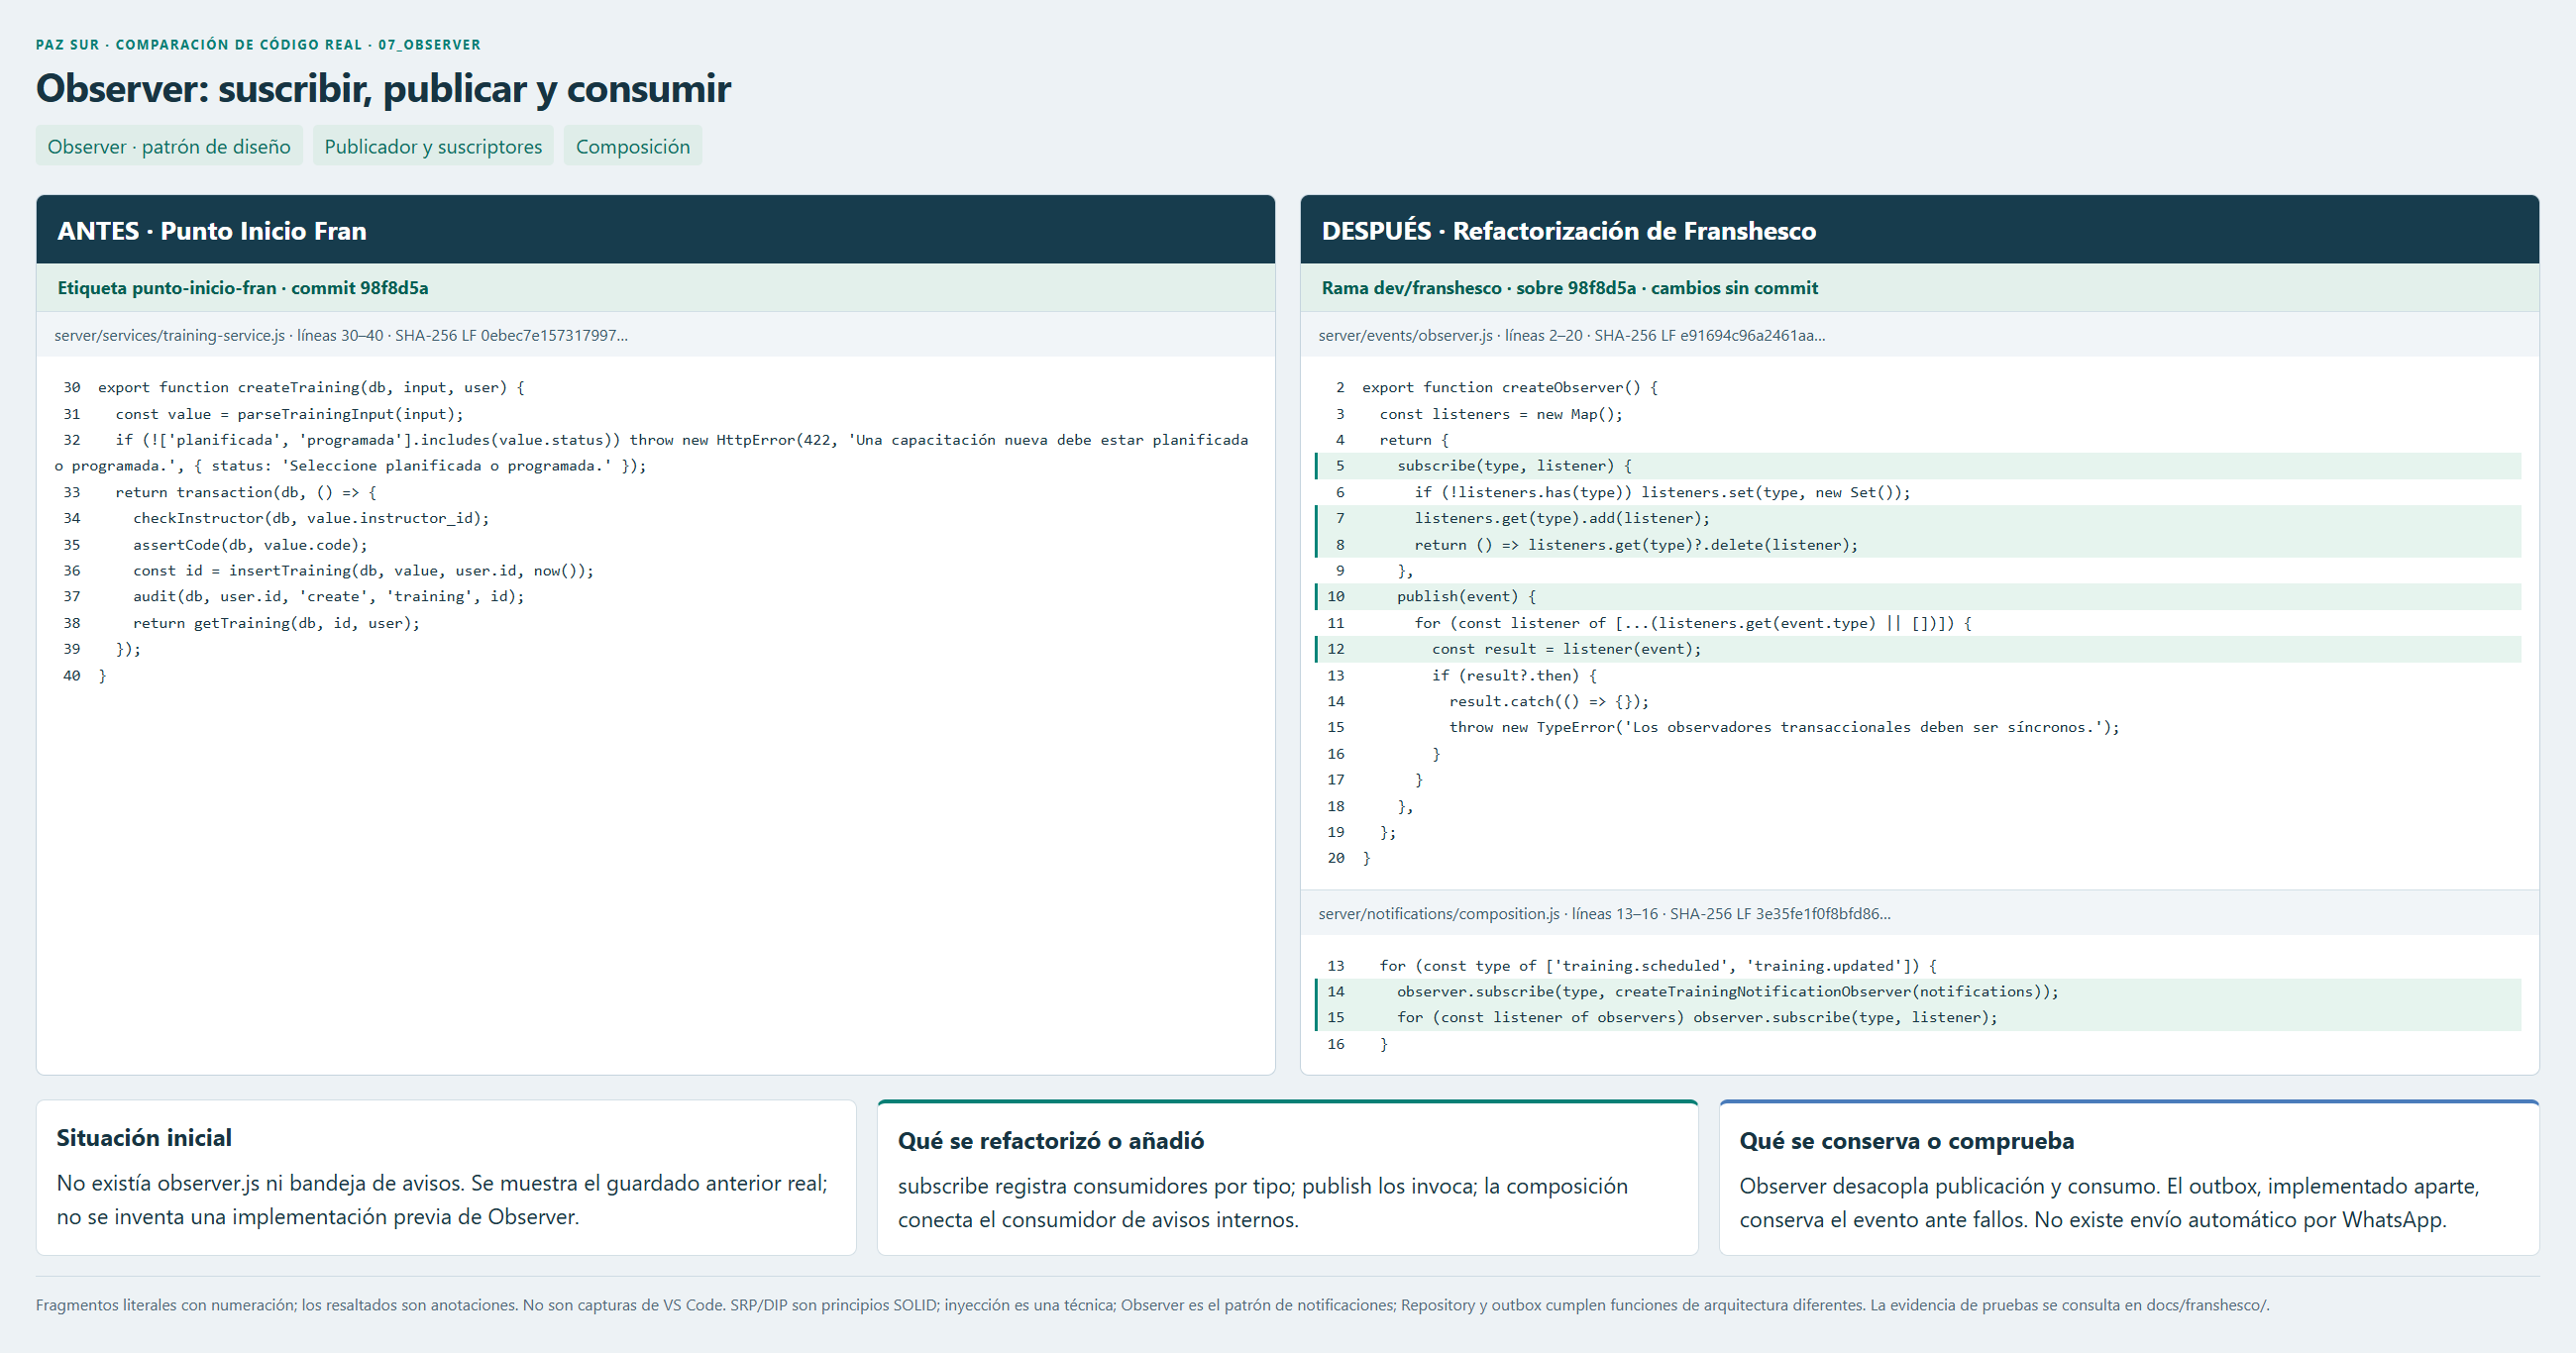
\includegraphics[width=\linewidth,height=0.82\textheight,keepaspectratio]{imagenes/franshesco/comparacion_codigo_07_observer.png}
\caption{Observer: guardado anterior frente al publicador y la suscripción reales de la versión nueva.}
\end{figure}

\section{Pruebas y resultados verificables}
Se usan bases en memoria o temporales con datos ficticios. La verificación final
se ejecuta sobre una copia aislada de la entrega, sin cargar el entorno privado ni
modificar la base de trabajo. También se evita sobrescribir las capturas históricas
de los compañeros al ejecutar sus pruebas de navegador.

\begin{center}\begin{tabular}{lrr}
\toprule Comprobación & Inicio & Refactorizado \\ \midrule
Pruebas backend, incluidos subcasos & 75 & 95 \\
Escenarios Chrome & 4 & 5 \\
Tipos TypeScript y build Vite & Aprobados & Aprobados \\
\bottomrule
\end{tabular}\end{center}

Las veinte pruebas nuevas de backend y el nuevo escenario de navegador amplían
la regresión. Los resultados no sustituyen revisión humana ni aceptación del cliente.

\begingroup\setlength{\parskip}{0pt}
\begin{table}[htbp]\centering\small
\begin{tabular}{P{0.30\textwidth}P{0.62\textwidth}}
\toprule Grupo & Casos relevantes \\ \midrule
Usuarios y DIP & Alta con colaboradores en memoria; dos altas simultáneas producen un solo registro; rollback completo si falla auditoría; página de 100 con cuatro SELECT. \\
Permisos y autenticación & Revocación durante hashing; autorización directa de roles; cambio de credenciales o desactivación durante login; hashes malformados y ventana de intentos. \\
Eventos y avisos & Suscripción/desuscripción, emisión correcta, PUT idéntico sin evento, fallos de auditoría o evento sin guardado parcial. \\
Recuperación y privacidad & Fallo de observador, reintento idempotente, pendiente tras reinicio, propiedad, CSRF y pérdida de acceso tras reasignación/revocación. \\
Navegador & Programación real, aviso visible, marcado como leído, persistencia al recargar y ancho móvil. \\
\bottomrule
\end{tabular}
\caption{Casos de prueba que sustentan las mejoras.}
\end{table}\endgroup

Los archivos propios de backend se encuentran en \path{tests/}:
\begin{itemize}
\item \path{franshesco-users.test.js}: usuarios, permisos e inyección.
\item \path{franshesco-auth.test.js}: autenticación y errores.
\item \path{franshesco-events.test.js}: eventos, avisos y recuperación.
\end{itemize}
El escenario de navegador se añade a \path{tests/ui.spec.ts}.
Los comandos reproducibles son:
\begin{lstlisting}[language={},numbers=none]
npm run check
npm run test:ui
node scripts/verify-franshesco.mjs
\end{lstlisting}
El último valida procedencia e integridad de imágenes y fragmentos; no reemplaza
las pruebas funcionales.

\section{Análisis de las evidencias de código y de interfaz}
La carpeta \path{docs/latex/imagenes/franshesco/} contiene 23 láminas:
\begin{itemize}
\item 14 archivos \texttt{comparacion\_visual\_*}, conservados intactos.
\item Nueve archivos \texttt{comparacion\_codigo\_*}, con ambos fragmentos juntos.
\end{itemize}
Se revisaron títulos, versiones, líneas, explicaciones y correspondencia con las
fuentes. Los hashes comprueban que las visuales no cambiaron y que el código
anterior procede de la etiqueta; el posterior coincide con los archivos de entrega.

\begingroup\setlength{\parskip}{0pt}
\begin{longtable}{P{0.28\textwidth}P{0.64\textwidth}}
\toprule Lámina de código & Evidencia que aporta \\ \midrule\endhead
01 Registro & Separación de responsabilidades y revalidación después del hash. \\
02 Autenticación & Extracción del caso de uso desde la ruta HTTP. \\
03 Permisos & Autorización dentro del servicio y escritura delegada. \\
04 Repository & SQL separado y recuperación por lotes. \\
05 Inyección & Relación entre contratos de colaboradores y composición concreta. \\
06 Eventos & Puerto de eventos conectado al guardado de capacitación. \\
07 Observer & Registro de suscriptores, publicación y consumidor concreto. \\
08 Outbox & Persistencia, rollback de avisos parciales y reintento. \\
09 Errores & Traducción de infraestructura y protección de detalles. \\
\bottomrule
\end{longtable}\endgroup

Las visuales 01--08 muestran continuidad de login, panel, usuarios y roles. Las
09--12 muestran programación, listado, edición y detalle de capacitaciones. La
13 demuestra la ampliación visible: antes se guardaba sin bandeja; después se
obtienen dos avisos por programar y modificar. La 14 compara el panel móvil previo
con la nueva bandeja; no se presenta como una pantalla de avisos que ya existiera.
La igualdad de diseño en formularios no prueba por sí sola SOLID ni seguridad:
esas mejoras se sustentan con código y pruebas.

Los rótulos ``cambios sin commit'' describen el momento real de captura anterior
al commit de entrega. Se conservan como evidencia histórica; no significan que la
rama publicada carezca de commit. Archivos, líneas y hashes vinculan esas capturas
con el código entregado. Los originales individuales están apartados en
\path{docs/franshesco/evidencias/archivo_png/}; los manifiestos y el índice permiten
ampliar cada PNG al 100\,\%. Las imágenes de código son transcripciones literales
anotadas, no capturas simuladas de VS Code.

\begin{figure}[p]\centering
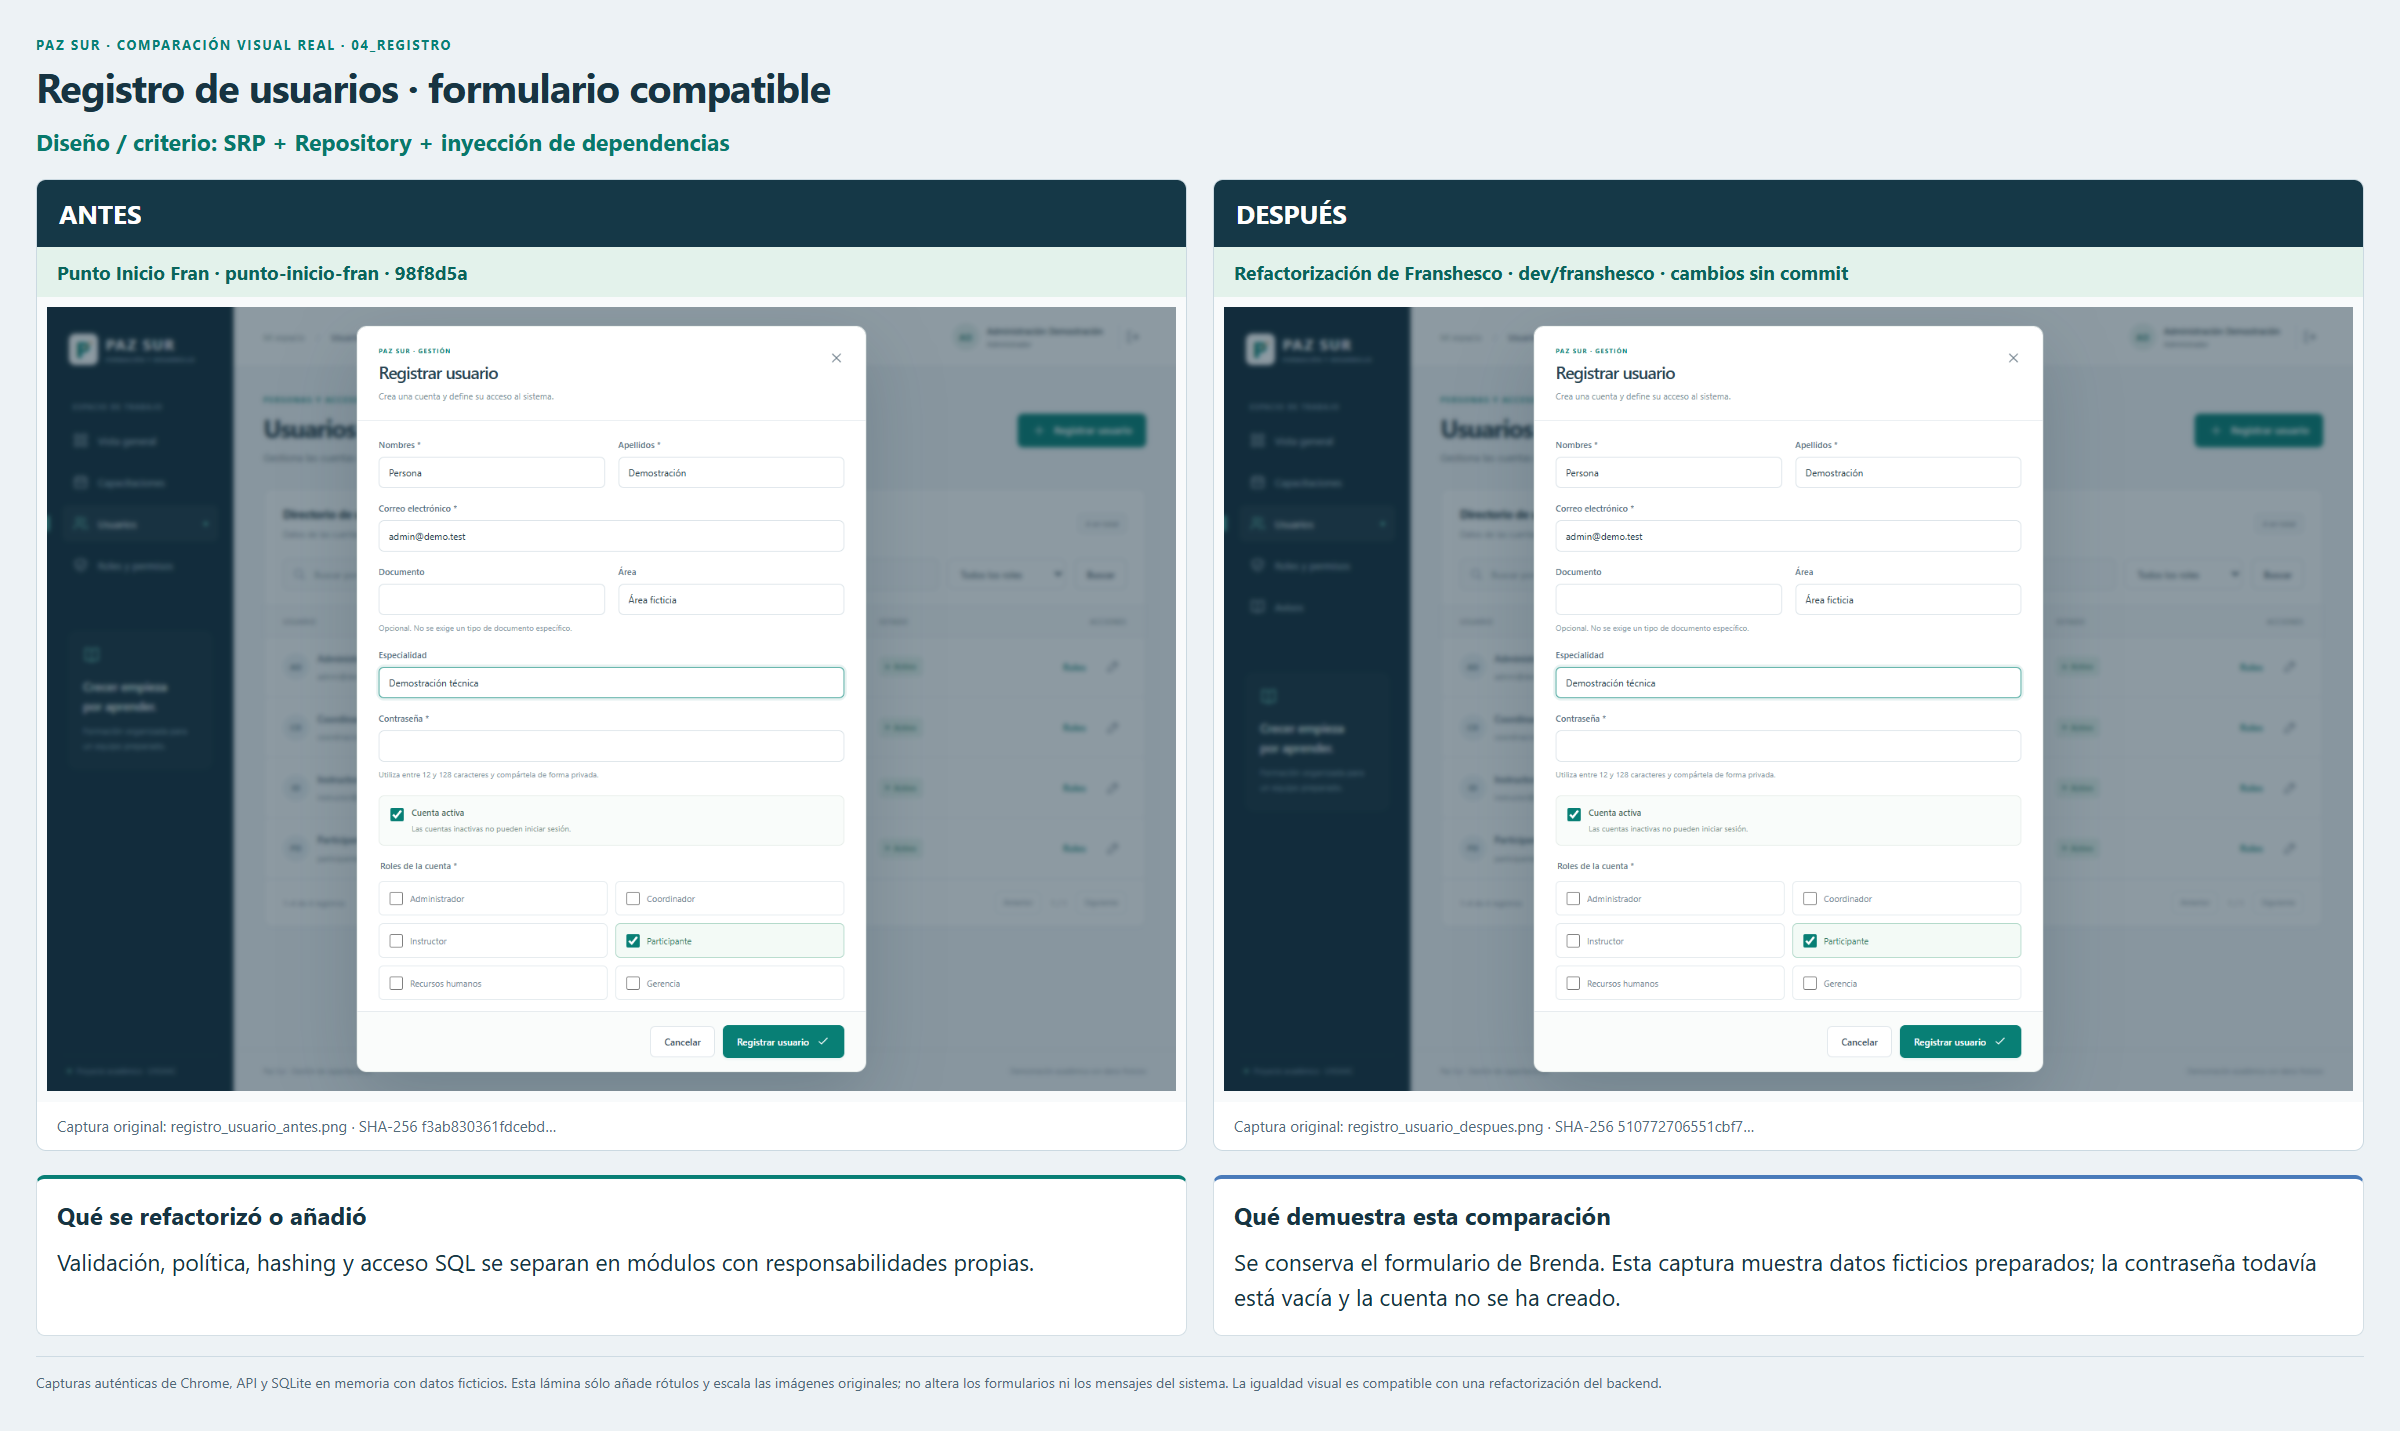
\includegraphics[width=\linewidth,height=0.82\textheight,keepaspectratio]{imagenes/franshesco/comparacion_visual_04_registro.png}
\caption{El formulario de Brenda se conserva: el cambio principal está en las responsabilidades del backend.}
\end{figure}
\begin{figure}[p]\centering
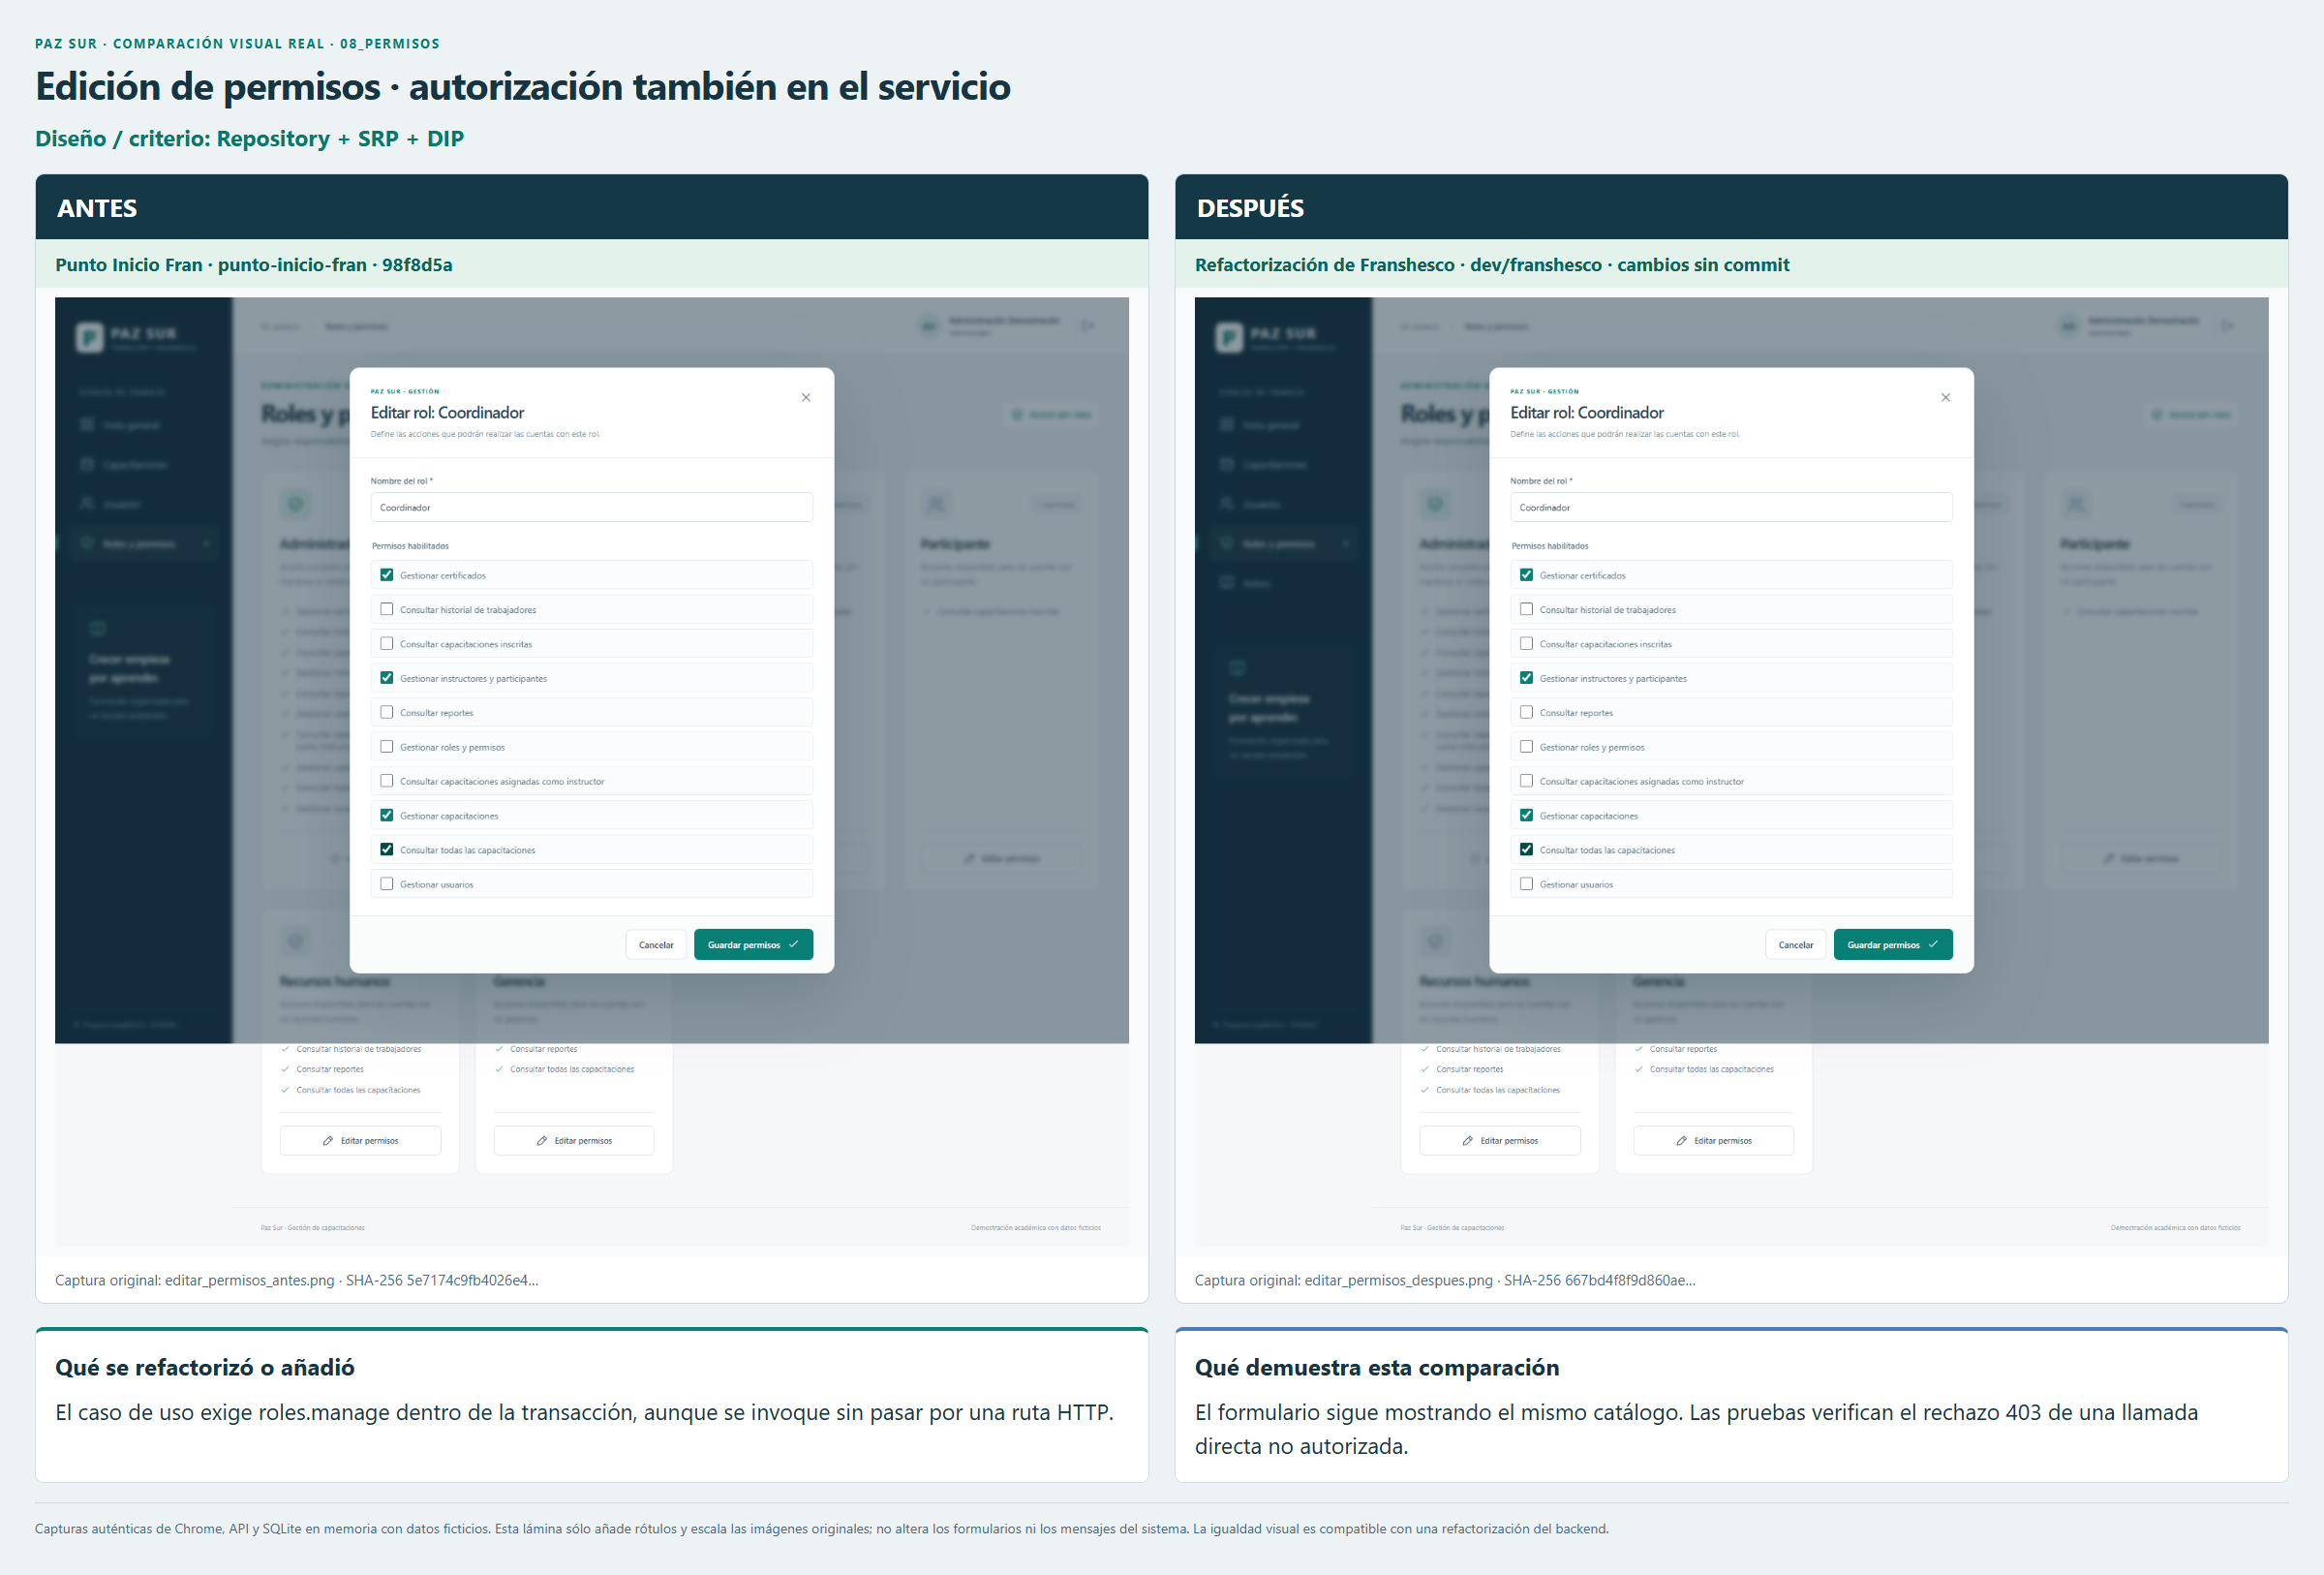
\includegraphics[width=\linewidth,height=0.82\textheight,keepaspectratio]{imagenes/franshesco/comparacion_visual_08_permisos.png}
\caption{Edición de permisos compatible con el servicio refactorizado. La autorización efectiva se acredita mediante pruebas adicionales.}
\end{figure}
\begin{figure}[p]\centering
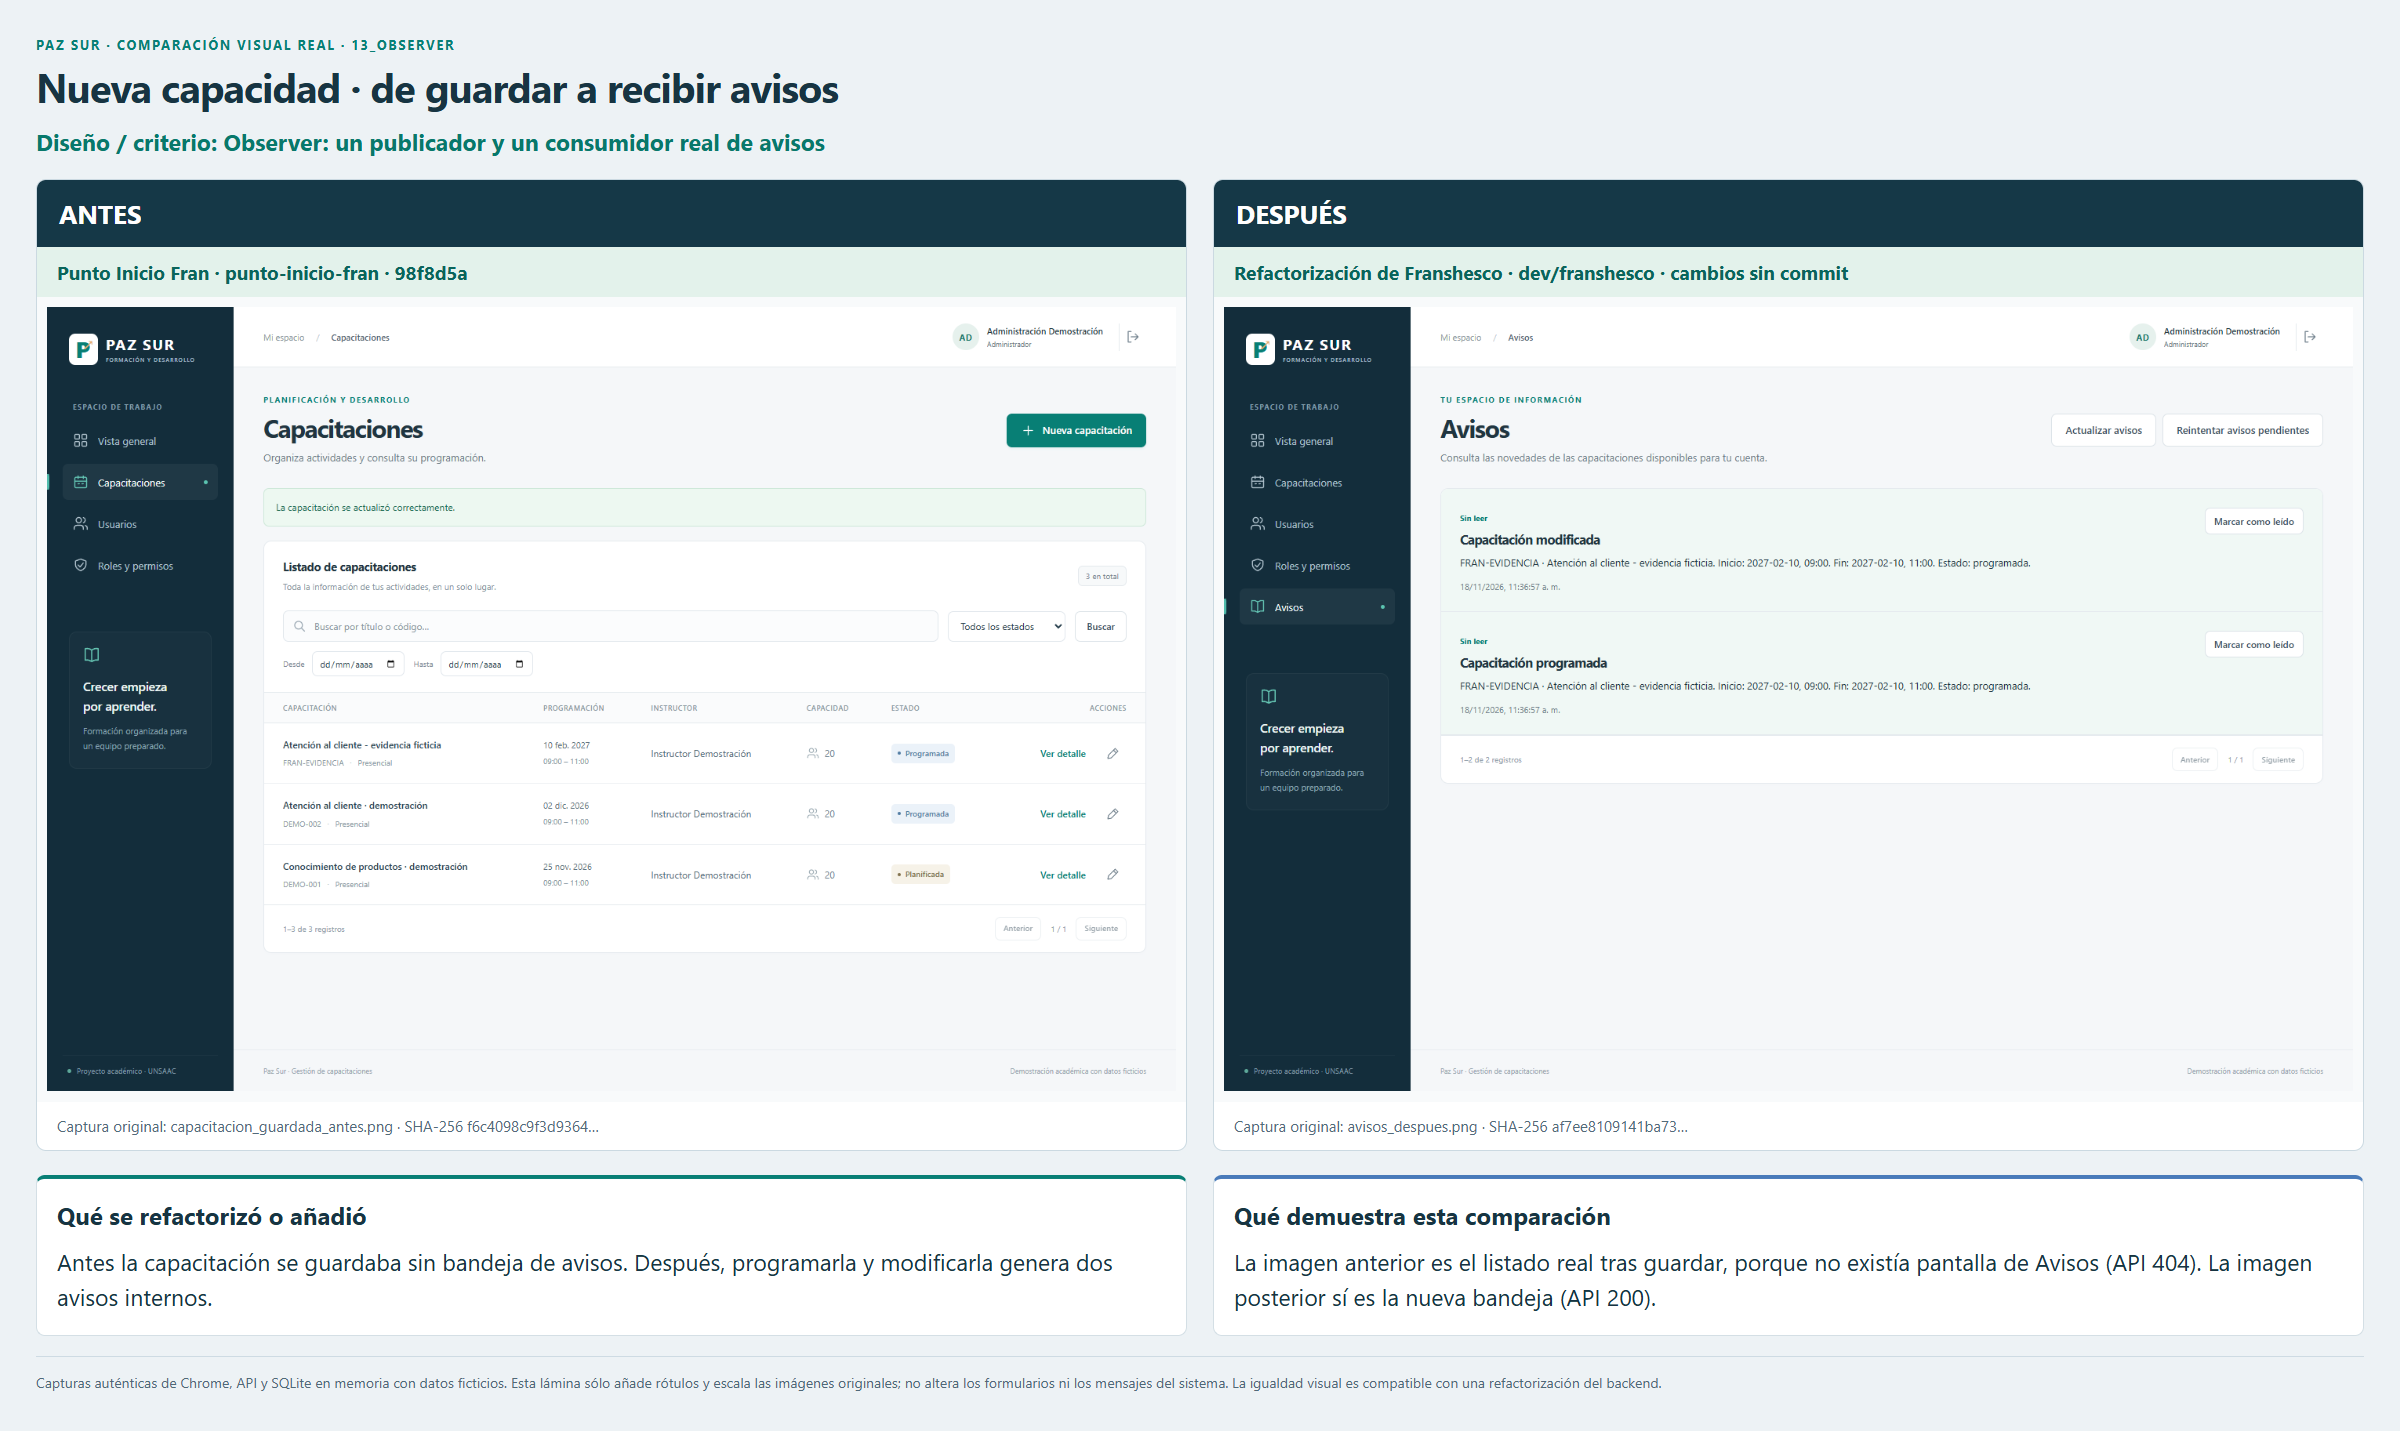
\includegraphics[width=\linewidth,height=0.82\textheight,keepaspectratio]{imagenes/franshesco/comparacion_visual_13_observer.png}
\caption{La nueva bandeja es un consumidor real de Observer; la referencia anterior no tenía ruta ni pantalla de avisos.}
\end{figure}
\clearpage

\section{Seguimiento del Sprint, integración y explicación final}
El tablero local \path{docs/franshesco/SPRINT.md} relaciona diagnóstico, refactorización,
pruebas y documentación con sus evidencias. La revisión realizada en el repositorio
no acredita reuniones, actualizaciones de Jira ni aprobaciones de otros integrantes.
Se propone revisión de compatibilidad con Brenda, de emisión de eventos con Adel
y del flujo de capacitación con Daniela, sin registrarlas como ya realizadas.

La entrega utiliza la rama \path{dev/franshesco} y el mensaje \texttt{Punto final fran 1}.
Publicar una rama no equivale a fusionarla con main, aprobar un Pull Request o
desplegar el sistema. Para demostrar el aporte se muestra la referencia inicial,
un fragmento anterior, el servicio actual y una prueba pertinente; después se
programa una capacitación, se modifica, se consultan los avisos y se marca uno
como leído. El guion completo está en \path{docs/franshesco/GUION_PROFESOR.md}.

El resultado defendible es una estructura de backend con responsabilidades más
cohesivas y dependencias explícitas, autorización reforzada y un consumidor de
eventos desacoplado. Observer es el patrón principal de notificaciones; Repository
y outbox apoyan persistencia y recuperación; SRP/DIP son principios y la inyección
es una técnica. State y Strategy no se añadieron a esta contribución.

Quedan por confirmar la política de destinatarios con Paz Sur, la revisión humana
y la integración por Pull Request. La funcionalidad de avisos es parcial respecto
a HU-26: no incluye inscritos, anticipación ni canales externos. Estos límites
evitan presentar el incremento como un producto completo o validado en producción.
